\chapter{Evaluation}

\section{Success criteria}

\paragraph{Success Criterion}
The original project proposal (\Aref{ch:proposal}) stated the following three criteria for success:
\begin{enumerate}
    \item 
        Implement SGC and extract the concepts used for each of the synthetic datasets.
        \label{crit1}
    \item 
        Implement GCN and extract the concepts to use as a baseline.
        \label{crit2}
    \item 
        Compare the concepts between SGC and GCN using the metrics of concept completeness and concept purity.
        \label{crit3}
\end{enumerate}

\emph{I completely meet all three success criteria.}
In addition to the above project success criteria, and to aid the analysis of SGC compared to GCN, 
I compare the two models to each other in mean \emph{test accuracy}.

\paragraph{Meeting criterion 1}
\note{reference the implementation.}
\Sref{sec:reproduction} verifies the correctness of the SGC implementation.
\Sref{sec:comp-concept} demonstrates concept extraction on the synthetic datasets.

\paragraph{Meeting criterion 2}
\note{reference the implementation.}
\Sref{sec:reproduction} verifies the correctness of the GCN implementation and demonstrates concept extraction.

\paragraph{Meeting criterion 3}
\note{reference the implementation.}
\Sref{sec:comp-concept} demonstrate the comparison of SGC and GCN using the metrics of concept completeness and purity.
Additionally, \Sref{sec:comp-acc} demonstrates further comparison between the models using the metric of model accuracy.

\section{Methodology}

\subsection{Hyperparameters}
\label{sec:hyperparameters}

\paragraph{Reproduction}
\textit{Magister et al.}\cite{magister2021gcexplainer} use a GCN model to evaluate their proposed graph concept explainer.
The paper trains and evaluates the model on the same 5 synthetic node classification datasets described in \Sref{sec:synth} and therefore the same hyperparameters are used for the GCN baseline.

\textit{Wu et al.}\cite{wu2019simplifying} states that the weight decay parameter for the Planetoid datasets was found using \texttt{hyperopt} over 60 iterations.
This process was repeated for results reproduction however it was found that the hyperparameters for the learning rate were different from those stated.

The hyperparameters for these models are available in tables \ref{tab:GCN-params} and \ref{tab:SGC-reproduction-params}.
Additionally the concept extraction metrics are presented in \ref{tab:GCN-concept-params}.

\begin{table}
    \centering
    \begin{tabular}{c|ccc}
        \textbf{Dataset} &
        \textbf{Layers} &
        \textbf{Learning rate} &
        \textbf{Epochs} \\
        \midrule
        BA Shapes       & 3 $\times$ 20 & 0.001 & 3000 \\
        BA Grid         & 3 $\times$ 20 & 0.001 & 3000 \\
        BA Community    & 6 $\times$ 50 & 0.001 & 6000 \\
        Tree Cycles     & 3 $\times$ 50 & 0.001 & 7000 \\
        Tree Grid       & 7 $\times$ 20 & 0.001 & 10000 \\
        \midrule \\
        REDDIT BINARY   & 4 $\times$ 40 & 0.005 & 3000 \\
        Mutagenicity    & 4 $\times$ 30 & 0.005 & 10000 \\
    \end{tabular}
    \caption{GCN hyperparameters from table 15 in \textit{Magister et al.}\cite{magister2021gcexplainer}. All models use \texttt{ReLU}\note{citation needed?} activation functions between layers with a single linear layer classifier with \texttt{softmax}\note{citation needed?}.}
    \label{tab:GCN-params}
\end{table}


\begin{table}[h]
    \centering
    \captionsetup{width=.9\textwidth}
    \begin{tabular}{c|cccc}
        \textbf{Dataset} &
        \textbf{Degree} &
        \textbf{Learning rate} &
        \textbf{Weight decay} &
        \textbf{Epochs} \\
        \midrule
        Cora        & 2 & 0.002 & 0.04 & 100 \\
        Citeseer    & 2 & 0.004 & 0.08 & 100 \\
        PubMed      & 2 & 0.0005 & 0.25 & 100 \\
    \end{tabular}
    \caption{SGC hyperparameters using \texttt{hyperopt}\cite{bergstra2013making} as proposed by \textit{Wu et al.}\cite{wu2019simplifying}. All models use \texttt{softmax}.}
    \label{tab:SGC-reproduction-params}
\end{table}


\begin{table}[h]
    \centering
    \captionsetup{width=.9\textwidth}
    \begin{tabular}{c|cc}
        \textbf{Dataset} &
        \textbf{Clusters (k)} &
        \textbf{Receptive field (n)} \\
        \midrule
        BA Shapes       & 10 & 2 \\
        BA Grid         & 10 & 3 \\
        BA Community    & 30 & 2 \\
        Tree Cycles     & 10 & 3 \\
        Tree Grid       & 10 & 3 \\
        \midrule
        REDDIT BINARY   & 20 & 1 \\
        Mutagenicity    & 30 & 3 \\
    \end{tabular}
    \caption{Concept extraction parameters used in \textit{Magister et al.}\cite{magister2021gcexplainer}.}
    \label{tab:GCN-concept-params}
\end{table}



\paragraph{New models}
This project proposes multiple new models designed for the different datasets.
The core project defines 5 models based on the SGC architecture as required by criterion \ref{crit1}.
As the underlying graph operator is the same for both GCN and SGC, as described in \Sref{sec:GCN} and \Sref{sec:SGC} the degree of the SGC model can be assumed to be the same as the GCN model for the same dataset.
This the same approach that \textit{Wu et al.}\cite{wu2019simplifying} take to creating there SGC models.

The learning rate for SGC models is likely to be different from the GCN models due to the reformulation.
Furthermore, \textit{Wu et al.}\cite{wu2019simplifying} use weight decay to keep weight values close to $0$ as would be assumed from the multiplication of weight matrices in equation \ref{eq:theta}.
Rather than use stochastic approaches to finding these hyperparameters a sweep of anticipated values is carried out.
This allows for a visualisation of the hyperparameter allowing for further exploration if necessary.
The learning rate is sampled from $\{0.01, 0.001, 0.0001\}$ and the weight decay from $\{1.0, 0.1, 0.01\}$.

The results of these searches is presented in figures \note{include the references the hyperparameter surfaces}.
As can be seen for the majority of hyperparameter searches the specific hyperparameters have minimal to no impact on the resulting model accuracy and therefore $0.01$ is chosen for learning rate and $0.1$ for weight decay.
The hyperparameters chosen are presented in table \ref{tab:SGC-params}

\begin{table}
    \centering
    \begin{tabular}{c|cccc}
        \textbf{Dataset} &
        \textbf{Degree} &
        \textbf{Learning rate} &
        \textbf{Weight decay} &
        \textbf{Epochs} \\
        \midrule
        BA Shapes       & 3 & 0.01 & 0.1 & 3000 \\
        BA Grid         & 3 & 0.01 & 0.1 & 3000 \\
        BA Community    & 6 & 0.001 & 0.1 & 6000 \\
        Tree Cycles     & 3 & 0.01 & 1.0 & 7000 \\
        Tree Grid       & 7 & 0.01 & 0.01 & 10000 \\
    \end{tabular}
    \caption{SGC hyperparameters based on the corresponding GCN hyperparameters in \ref{tab:GCN-params} and using the results of the hyperparameter search in \note{reference when added}. All models use \texttt{softmax}\note{citation needed?}.}
    \label{tab:SGC-params}
\end{table}



\paragraph{Datasets}
The batch sizes for all the datasets match those described in \textit{Ying et al.}\cite{ying2019gnnexplainer} and \textit{Kipf et al.}\cite{kipf2016semi}.
The number of epochs for each dataset matches those proposed in \textit{Magister et al.}\cite{magister2021gcexplainer} and \textit{Wu et al.}\cite{wu2019simplifying} or until convergence for SGC.

\subsection{Model Evaluation}
\label{sec:evaluation}

\paragraph{Concept evaluation}
Criterion \ref{crit3} requires evaluation of the models with respect to concept purity and completeness.
These metrics are discussed in \ref{sec:GCE} and implementation is described in \note{reference when complete}.
On top of the quantitative analysis of the different models concepts lend themselves to qualitative analysis which will mainly focus on visual similarities between the two models.
the quantitative analysis will also help to infer the differences in how the two models infer labels on the input data.

For qualitative analysis only BA Shapes and Mutagenicity will be covered in detail with brief analysis of the other datasets in Appendix \note{reference when complete}.
This extends to extensions where only BA Shapes and Mutagenicity are trained on as proofs of concepts.

It is important to note a number of drawbacks of the GCExplainer in comparing two different models quantitatively.
\begin{enumerate}
    \item 
        Concept purity is calculated only using subgraphs with less than 13 nodes.
        This means that pure quantitative analysis does not represent a full comparison of the two models.
    \item 
        The number of clusters and the receptive field of the concepts can be arbitrarily manipulated to find the highest score.
        To combat this the new SGC models are compared against the same concept extraction parameters presented in table \note{reference when completed}.
    \item 
        \label{nb:accuracy}
        \textit{Ying et al.}\cite{ying2019gnnexplainer} only suggest concept extraction for models that achieve an accuracy of atleast $95\%$ on synthetic datasets. 
\end{enumerate}

The full comparison of concepts requires a qualitative analysis of the extracted concepts.
The concepts produced by SGC can be analysed in isolation to infer how SGC reasons about graphs.
These can then be compared to the concepts produced by GCN to highlight the differences in reasoning and which is easier to understand.
When reproducing results this is done by comparing the analysis suggested by \textit{Magister et al.}\cite{magister2021gcexplainer} to the reproduced concepts.
Furthermore, a visual comparison of the concepts can be made, such as matching published concepts to reproduced concepts.

\paragraph{Accuracy evaluation}
Drawback \ref{nb:accuracy} motivates the additional evaluation metric of accuracy as \Sref{sec:comp-acc} demonstrates that SGC does not meet the desired accuracy.
To evaluate this each synthetic dataset is split into a train and test set using an 80:20 split.
Note that TUDataset\note{citation needed} and Planetoid\note{citation needed} use there own train/test splits.

The synthetic datasets are generated randomly along with the train/test split and thus each random seed produces a new variation of the synthetic dataset.
This means that using the same seeds across different models for the experiments results in the same train/test split.
This also means that although the hyperparameter search evaluates parameters on the test split of the dataset using a different seed to the experiments means that the experiment test splits are effectively unseen.

\subsection{Confidence intervals}
\label{sec:reporting}
The mean accuracy across 10 different initiliasations is reported using $\mu = \sum_i\frac{\text{accuracy}_i}{10}$ as an unbiased estimator of the mean.
The confidence interval of each of the runs uses the unbiased standard deviation estimator $\sigma = \sqrt{\sum_i(\text{accuracy}_i - \mu)/(10 - 1)}$.
For experiments where very high variance is present outliers are removed based on the median, $m$, and the interquartile range, $\text{ITR}$, of the accuracies.\footnote{In the cases where outliers are removed the estimators are adjusted accordingly.}
An outlier is defining as being outside the range $[m - 1.5 \times \text{ITR}, m + 1.5 \times \text{ITR}]$.


\subsection{Reproducibility}
\error{Return to at the end to make sure that all aspects are met.}

\subsection{System specifications}
The experiments are not resource-intensive due to the incredibly small datasets and so carrying out the hyperparameter search and multiple final runs can be completed on my personal machine.
My machine has an AMD Ryzen 7 5700U CPUs @ 1.8GHz with 16 cores wuth 15 Gigabytes of RAM.
The machine does have an AMD ATI Lucienne GPU but due to the fact that \texttt{PyTorch Geometric}\note{citation needed} did not support RoCM I was unable to utilise this.

To speed up the retrieval of experimental results for extensions I utilised a Google Colab Pro account with 1 hyperthreaded Intel Xeon Processor @ 2.3GHz with 1 core and 12 Gigabytes of Ram.
The account also has access to a Tesla K80 GPU with 12GB of RAM.

\note{Include figures demonstrating system use later.}

\section{Results Reproduction}
\label{sec:reproduction}

As discussed in \Sref{sec:testing} the testing strategy includes the reproduction of prior results from \textit{Magister et al.}\cite{magister2021gcexplainer} on GCN and \textit{Wu et al.}\cite{wu2019simplifying} on SGC.
I reproduce all of the experiments from \textit{Magister et al.} and the Planetoid\cite{kipf2016semi} from \textit{Wu et al.} as these are most relevant.

\paragraph{Success criterion}
\Sref{sec:GCN-reproduction} demonstrates an implementation of GCN trained on the synthetic datasets with concept extraction.
Tables \ref{tab:GCN-acc} and \ref{tab:GCN-concepts} and figure \ref{fig:GCN-BA-Shapes} demonstrate the results achieved.
This fulfills the \ref{crit2}$^{nd}$ success criterion.

\paragraph{Method}
In both cases across all datasets the hyperparameters presented in tables \ref{tab:GCN-params} and \ref{tab:SGC-reproduction-params} are used.
Each model, dataset experiment is run 10 times with different randomly pre-selected seeds and the mean and confidence interval are presented in accordance with \Sref{sec:reporting}.
The implementation of SGC is the one presented in \note{reference section when complete} and the implementation of GCN uses the layers provided by \texttt{PyTorch Geometric}\cite{Fey/Lenssen/2019}.

\subsection{SGC}
\begin{table}
    \centering
    \begin{tabular}{c|cc}
        \multicolumn{1}{c}{\textbf{Dataset}} &
        \multicolumn{1}{c}{\textbf{Wu et al.}} &
        \multicolumn{1}{c}{\textbf{My results}} \\
        \midrule
        Cora        & 81.0\% $\pm$ 0.0 & 80.0\% $\pm$ 0.1 \\
        Citeseer    & 71.9\% $\pm$ 0.1 & 71.4\% $\pm$ 0.1 \\
        Pubmed      & 78.9\% $\pm$ 0.0 & 71.3\% $\pm$ 2.1 \\
    \end{tabular}
    \caption{Reproduction of experiments from table 2 in \textit{Wu et al.}\cite{wu2019simplifying}. The mean accuracy of 10 experiment runs is taken using hyperparameters found by \texttt{hyperopt}\note{citation needed}.}
    \label{tab:SGC-reproduction}
\end{table}



Table \ref{tab:SGC-reproduction} presents the accuracy achieved by my SGC models compared to the accuracy presented in table 2 of \textit{Wu et al.}\cite{wu2019simplifying}.
As can be seen in both Cora and Citeseer the accuracies are closely correlated, though the accuracy presented by \textit{Wu et al.} are outside of my confidence interval.
Comparitively Pubmed presents a large discrepancy between the published results and the reproduced results with large variation in the reproduced results.
These descrepancies are likely due to the uncertainty in hyperparameters as the exact weight decay constant used is unknown.
Furthermore, the published learning rate of 0.2 yields worse results and so, as demonstrated in table \ref{tab:SGC-reproduction-params}, new learning rates are used.
Based on these considerations I consider my implementation of SGC to be correct.

\subsection{GCN}
\label{sec:GCN-reproduction}
\paragraph{Accuracy}
\begin{table}
    \centering
    \begin{tabular}{c|cc}
        \multicolumn{1}{c}{\textbf{Dataset}} &
        \multicolumn{1}{c}{\textbf{Magister et al.}} &
        \multicolumn{1}{c}{\textbf{My results}} \\
        \midrule
        BA Shapes       & 95.6\% & 98.0\% $\pm$ 2.2 \\
        BA Grid         & 99.0\% & 99.5\% $\pm$ 0.7 \\
        BA Community    & 95.7\% & 86.3\%\tablefootnote{\label{nb:epochs1}Using the same epochs stated in \textit{Magister et al.}\cite{magister2021gcexplainer}. More epochs yields a closer value.} $\pm$ 3.3 \\
        Tree Cycles     & 96.0\% & 95.8\% $\pm$ 3.2 \\
        Tree Grid       & 95.1\% & 92.5\% $\pm$ 5.4 \\
        \midrule
        REDDIT BINARY   & 89.1\% & 89.1\% $\pm$ 2.2 \\
        Mutagenicity    & 93.0\% & 93.8\% $\pm$ 1.6 \\
    \end{tabular}
    \caption{Reproduction of experiments from table 16 in \textit{Magister et al.}\cite{magister2021gcexplainer}. The mean test accuracy of 10 experiment runs is taken using \textit{Magister et al.}'s hyperparameters.}
    \label{tab:GCN-acc}
\end{table}


Table \ref{tab:GCN-acc} presents the accuracy achieved my GCN models compared to the accuracy published in table 16 of \textit{Magister et al.}\cite{magister2021gcexplainer}.
As can be seen in the majority of cases the reproduced accuracy matches or exceeds the accuracy presented by \textit{Magister et al.}.
Given the small size of the synthetic datasets it is expected that close to 100\% accuracy is achieved which is demonstrated in all but BA Community.
For the real-world datasets the expectation is above 85\% as suggested by \textit{Ying et al.}\cite{ying2019gnnexplainer}.

BA Community is a significant outlier in the results neither reaching the suggested 95\% or reaching a value close to 100\%.
If the model is allowed to train for more than the defined 6000 epochs an accuracy closer to 95\% is achieved.
A likely cause for this discrepancy is the uncertainty in the construction of the community dataset discussed in \note{reference when complete}.
Due to these considerations I consider my implementation of GCN to be correct.

\paragraph{Concept scores}
\begin{table}
    \centering
    \begin{tabular}{c|cccc}
        \multirow{2}{*}{\textbf{Dataset}} &
        \multicolumn{2}{c}{\textbf{Magister et al.}} &
        \multicolumn{2}{c}{\textbf{My results}} \\
        &
        \textbf{Completeness} & 
        \textbf{Purity} & 
        \textbf{Completeness} & 
        \textbf{Purity} \\
        \midrule
        BA Shapes       & 0.964 & 3.375 & 0.929 & 0.000 \\
        BA Grid         & 1.000 & 4.923 & 1.000 & 0.000 \\
        BA Community    & 0.678 & 0.000 & 0.623 & 5.600 \\
        Tree Cycles     & 0.949 & 1.167 & 0.970 & 4.391\\
        Tree Grid       & 0.965 & 3.100 & 0.951 & 1.417\\
        \midrule
        REDDIT BINARY   & 0.713 & 6.968 & 0.746 & 1.429 \\
        Mutagenicity    & 0.967 & 5.400 & 0.626 & 0.375 \\
    \end{tabular}
    \caption{Reproduction of experiments from tables 4 and 5 in \textit{Magister et al.}\cite{magister2021gcexplainer}. The activation space for each experiment selected from the best performing model is used with the mean purity score presented.}
    \label{tab:GCN-concepts}
\end{table}


Table \ref{tab:GCN-concepts} presents the concept scores for each of the top performing GCN models compared to those in tables 4 and 5 in \textit{Magister et al.}.
Only the mean purity is presented across all the models with the minimum and maximum purity available in table \note{reference when complete}. As with the accuracy reproduction the values for concept completeness are closely correlated for the majority of the models.

\fig{erroneous-labels}{A subset of the concepts discovered for Mutagenicity highlighting the erroneous labels. Each row represents a concept and the graphs are coloured according to standard chemical colouring \note{citation needed}.}

Figure \ref{fig:erroneous-labels} demonstrates that the clustering for Mutagenicity focuses on chemical similarity which does not correlate to mutagen similarity.
This means that the concept completeness is likely to be low as demonstrated in \ref{tab:GCN-concepts} though the actual model accuracy may be high.

The average purity is far more erratic with little correlation between the two results which would suggest that the purity score or concept extraction is incorrect.
However, the 13 node cut-off and non-deterministic nature of k-Means\note{citation needed} clustering is likely to be the cause rather than an incorrect implementation.

\fig{GCN-BA-Shapes}{A subset of concepts discovered for BA-Shapes from the best perfomring GCN model. Green nodes highlight the node of interest and pink nodes highlight the neighbourhood used for inference. Each row represents an individual concept.}

\fig{Magister-BA-Shapes}{A subset of the BA Shapes concepts discovered in figures 2, 3 and 5 from \textit{Magister et al.}\cite{magister2021gcexplainer} to demonstrate the full range of labels. Each row represents an individual concept, the same colour system is used as fig. \ref{fig:GCN-BA-Shapes}.}

Figure \ref{fig:GCN-BA-Shapes} presents a subset of the BA Shapes concepts reproduced by the best performing GCN model.
For comparison figure \ref{fig:Magister-BA-Shapes} presents those published in \textit{Magister et al.}
Concept 1 and A are included to demonstrate that the model does identify the base graph, in this case Barabasi-Albert, but as can be seen this provides little insight into how the model reasons.
The remaining concepts demonstrate the 3 other labels associated with the house motif, as discussed in \Sref{sec:synth}.

As can be seen all the published concepts have an equivalent concept in the reproduced concepts.
The same analysis can be made that the edge attaching the house motif to the base graph is important to the classification of the nodes.
There is also the same distinction between concepts 2 and 3 as concepts B and C representing ``inside'' and the ``outside'' nodes respectively.
Notice that in both concept 2 and B the  ``inside'' node clearly attaches to the Barabasi-Albert base graph.
This distinction is also present in concept 4 and D, with both the published and reproduced concepts focusing on the ``inside'' bottom node.

In both cases, and as expected given the concept purity scores, the concepts related to the motifs are almost completely pure with the exception of concept 1 and B.
Additionally, all the nodes in the house motif have a unique concept where applicable and this leads to the high completeness score.

Given the visual similarity in concepts between the published and reproduced results I consider the implementation of GCN to be accurate.
Examples of the other synthetic and real datasets is available in Appendix \note{reference when complete}.
\note{There may also be brief comparisons between the figures time permitting.}

\section{Comparison of Accuracy}
\label{sec:comp-acc}
\begin{table}
    \centering
    \begin{tabular}{c|c}
        \textbf{Dataset} & \textbf{Accuracy} \\
        \midrule
        BA Shapes       & 61.4\% $\pm$ 3.3 \\
        BA Grid         & 72.4\% $\pm$ 1.6 \\
        BA Community    & 20.6\% $\pm$ 1.5 \\
        Tree Cycles     & 50.5\% $\pm$ 4.2 \\
        Tree Grid       & 59.2\% $\pm$ 1.6 \\
    \end{tabular}
    \caption{Test accuracy in \% of SGC on each of the synthetic datasets using the hyperparameters in table \ref{tab:SGC-params}. As per \textit{Wu et al.}\cite{wu2019simplifying} outliers are removed as defined in \note{reference when complete}.}
    \label{tab:GCN-acc}
\end{table}



Table \ref{tab:SGC-acc} demonstrates the mean accuracies achieved by each of the SGC models using the hyperparameters in \ref{tab:SGC-params}.
As a comparison the accuracies achieved by GCN are presented beside them.
The performanace of SGC is very poor and so random guesses are included as well to demonstrate the limited inference of SGC.

\paragraph{Compared to GCN}
the accuracies achieved by SGC are significantly worse and go against \textit{Wu et al.}'s claim that SGC can match GCN perfomance.
In the cases of the Tree datasets GCN nearly doubles the accuracy and in the case of BA Community GCN is more than $4\times$ as accurate.
Only in the case of BA Grid does SGC achieve a good accuracy in comparison to GCN though even here the difference in accuracy is $27.1$\%.

These poor results suggest that the graph structure inference of SGC is far worse than that of GCN as labels are based only on graph structure.
This is also an explanation for why SGC is able to surpass the accuracy of GCN in the Planetoid\cite{Fey/Lenssen/2019} as these datasets rely heavily on node representations.

\paragraph{Compared to random guesses}
SGC does not perform much better except in the cases of BA Shapes and BA Grid.
In the cases of the Tree datasets this can be attributed to the sparsity of the base graph resulting in less information being aggregated in the pre-computation stage.
Especially in the case of Tree Cycles where the Cycle structure and BST structure share similar sparse connections.

Comparatively the dense BA graph allows for a better distinction between the motifs and the base graph.
This distinction based on degree is attributed to the degree normalisation demonstrated in equation \ref{eq:GCN-as-GNN}.
This advantage is not present in BA Community because of the increase in classes, the need to distinguish the two communities and the possibility of a motif having multiple connections to different base graphs.

These poor results are not due to poor hyperparameter selection as is demonstrated in Appendix \note{reference when complete} and discussed in \Sref{sec:hyperparameters}.
Instead the explanation for the poor performance is due to the lack of proper graph structure inference in SGC.
This is lack of graph structure inference is not in comparison to GCN but rather a fundamental property of SGC.

\paragraph{Comparison of parameters}
Given that SGC uses a single linear regressor compared to GCNs multiple layers there is a large discrepancy in number of parameters.
SGC has $\sim40$ parameters compared to GCN with 1000+ for BA Shapes which is very significant difference.
However, increasing the parameters for SGC by increasing the node feature size and adding a \emph{multi-layer perceptron}(MLP) with the same hidden layers as the GCN model results in no substantial change to accuracy.

No MLP model is added before the SGC pre-computation step as this defeats the point of SGC to be linear.\footnote{The use of an MLP classifier also introduces non-linearity though in this case the model does not improve. Non-linearity and parameters on there own are not sufficient.}
This is the main drawback of SGC as it cannot manipulate the node representations beyond simple message passing/filter application.
\Sref{sec:comp-concept} explores these claims further demonstrating the importance of trainable parameters during message and non-linearity.

\section{Comparison of concepts}
\label{sec:comp-concept}

To achieve the \ref{crit1}$^{st}$ and \ref{crit3}$^{rd}$ success criterion concepts need to be extracted from SGC and compared to GCN concepts.
However, as stated before, concept extraction and analysis is only suggested for models that achieved $95$\% or higher on synthetic datasets by \textit{Ying et al.}\cite{ying2019gnnexplainer}.
As demonstrated in \Sref{sec:comp-acc} SGC does not reach this value only reaching $72.4$\% in the best case.

However, though the concepts will not be meaningful to explain how SGC reasons they will still provide insight into the claims in \Sref{sec:comp-acc}.
Furthermore, the concepts highlight the shortcomings of SGC when it comes to graph structure inference.
For this reason the analysis of the concept scores is limited but the qualitative concept analysis provides insight into where SGC fails.

\paragraph{Success criterion}
Table \ref{tab:SGC-acc} demonstrates and implementation of SGC trained on the synthetic datasets with tables \ref{tab:SGC-completeness} and \ref{tab:SGC-purity} showing concept extraction.
Figures \ref{fig:SGC-BA-Shapes} and \ref{fig:BA-Community} visualise the extracted concepts from the relevant SGC model. These fulfill the \ref{crit1}$^{st}$ success criterion.

Table \ref{tab:SGC-completeness} and \ref{tab:SGC-purity} also include a comparison to the scores achieved by GCN.
\Sref{sec:comp-concept} includes a detailed analysis of the concepts extracted for SGC and comparison to those extracted for GCN.
These fullfil the \ref{crit3}$^{rd}$ success criterion.

\subsection{Quantitative analysis}
\label{sec:quant}
\paragraph{Completeness}
\begin{table}
    \centering
    \begin{tabular}{c|c|c}
        \textbf{Dataset} &
        \textbf{SGC} &
        \textbf{GCN} \\
        \midrule
        BA Shapes       & 0.882 & 0.964 \\
        BA Grid         & 0.843 & 1.000 \\
        BA Community    & 0.264 & 0.678 \\
        Tree Cycles     & 0.874 & 0.949 \\
        Tree Grid       & 0.890 & 0.965 \\
        \midrule
        Mutagenicity    & 0.537 & 0.967 \\
    \end{tabular}
    \caption{Concept completeness scores of SGC on each of the synthetic datasets using the hyperparameters in table \ref{tab:SGC-params} compared to the completeness scores of the equivalent GCN models.}
    \label{tab:SGC-completeness}
\end{table}



Table \ref{tab:SGC-completeness} demonstrates the completeness scores achieved by SGC compared to GCN and as expected, by the low accuracy achieved by SGC in \Sref{sec:comp-acc}, they are consistently lower than the equivalent GCN models.
However, given the accuracies of SGC appears closs to random, the resulting completeness scores aresurprisingly close to the GCN scores except in the case of BA Community.

The high completenes scores are due to the fact that completeness relates to importance of concepts and not the performance of the model.
The relatively high completeness scores for SGC signify that the concepts that SGC produces have some relevance to the class of a node.
However, as demonstrated by table \ref{tab:SGC-completeness}, this relevance is not as strong as that in GCN.

\paragraph{Purity}
\begin{table}
    \centering
    \begin{tabular}{c|ccc|c}
        \multirow{2}{*}{\textbf{Dataset}} &
        \multicolumn{3}{c}{\textbf{SGC}} & \\
        & \textbf{Max.} & \textbf{Min.} & \textbf{Mean} & \multirow{-2}{*}{\textbf{GCN}}\\
        \midrule
        BA Shapes       & 0.0 & 4.0 & 0.8 (5) & 0.000 (4) \\
        BA Grid         & 0.0 & 0.0 & 0.0 (2) & 0.000 (2) \\
        BA Community    & 0.0 & 6.0 & 4.0 (4) & 5.600 (3) \\
        Tree Cycles     & 0.0 & 6.0 & 1.0 (6) & 4.391 (9) \\
        Tree Grid       & 0.0 & 7.0 & 3.3 (10) & 1.417 (6) \\
    \end{tabular}
    \caption{Concept purity of SGC on each of the synthetic datasets using the hyperparameters in table \ref{tab:SGC-params} compared to the average purity achieved by the equivalent GCN model. The brackets represent the number of concepts considered for purity, as per \Sref{sec:evaluation} these are graphs with less than 13.}
    \label{tab:SGC-purity}
\end{table}



Table \ref{tab:SGC-purity} demonstrates the purity scores achieved by the best performing SGC model compared to GCN.
As discussed in \Sref{sec:GCN-reproduction} the values for purity are likely to be very erratic and not well suited for direct comparison.
Given this erratic behaviour the values for purity between the two approaches are somewhat correlated with SGC achieving fairly pure concepts.
As demonstrated SGC can identify pure concepts as is the case of BA Grid, which matches GCN in completely pure concepts.\footnote{For subgraphs the contain less than 13 nodes.}

However, the inclusion of the number of concepts considered when calculating purity demonstrates the limitation of this method of comparison.
Due to the base graphs a number of concepts contain more than 13 nodes and therefore are not considered.
Thus the pure concepts of BA Grid are not representative of all the concepts extracted.

Overall, this demonstrates that though SGC does not perform as well as GCN it produces concepts that are as coherent as GCN produces.

\subsection{Qualitative analysis}
\label{sec:concept-analysis}

\paragraph{BA Shapes}
\fig{SGC-BA-Shapes}{A subset of concepts extracted from the best performing SGC model. The subset includes both pure and impure concepts. The same colour scheme as fig. \ref{fig:GCN-BA-Shapes} is used.}

Figure \ref{fig:SGC-BA-Shapes} visualises a subset of the concepts extracted for SGC on BA Shapes.
Concepts 1 to 4 demonstrate the purer concepts extracted for SGC with concepts 5 to 7 representing the more common impure concepts extracted.
Concept 5 demonstrates a shortcoming of the approach to calculating purity as this is considered a ``pure'' concept as the Barabasi-Albert graphs are not considered when calculating the score. 
As with GCN, concept 1 demonstrates that SGC is able to identify the base graph consistently but as stated in \Sref{sec:GCN-reproduction} this provides little insight into the behaviour of SGC.

Concepts 2, 3 and 4 demonstrate that SGC can identify pure concepts with important graph structure components.
These concepts can be directly compared to concepts 3, 2 and 4 in figure \ref{fig:GCN-BA-Shapes} respectively.
As with GCN the attaching arm is important to the classification of the nodes and there is some distinction in concept 2 and 3 between ``inside'' and ``outside'' middle nodes.
However, as can be seen in concept 2, this distinction is not as strong as GCN.

Concepts 5, 6 and 7 demonstrate the common impure concepts that are extracted from SGC.
This is the major shortcoming of SGC even with the large differences in degree if cannot consistently distinguish between the base graph and the motif.
Given that the nodes of interest in house motif are all consistent across these concepts suggests that there is an element of structure being identified.
The problem is that SGC is unable to discern between structures that produce similar node representations.

This observation suggests that the main shortcoming of SGC is the lack of learnable influence on node representations.
In comparison GCN allows for manipulation of the node representations as demonstrated by $\bm{\Theta}^{(l)}$ in equation \ref{eq:GCN1}.
Though equation \ref{eq:theta} suggests this manipulation should be preserved the reality is that only the final filter output is manipulated.
This observation leads to the extension presented in \Sref{sec:Jump-SGC} allowing SGC to access individual filter applications.

\paragraph{BA Community}
\begin{figure}
    \centering
    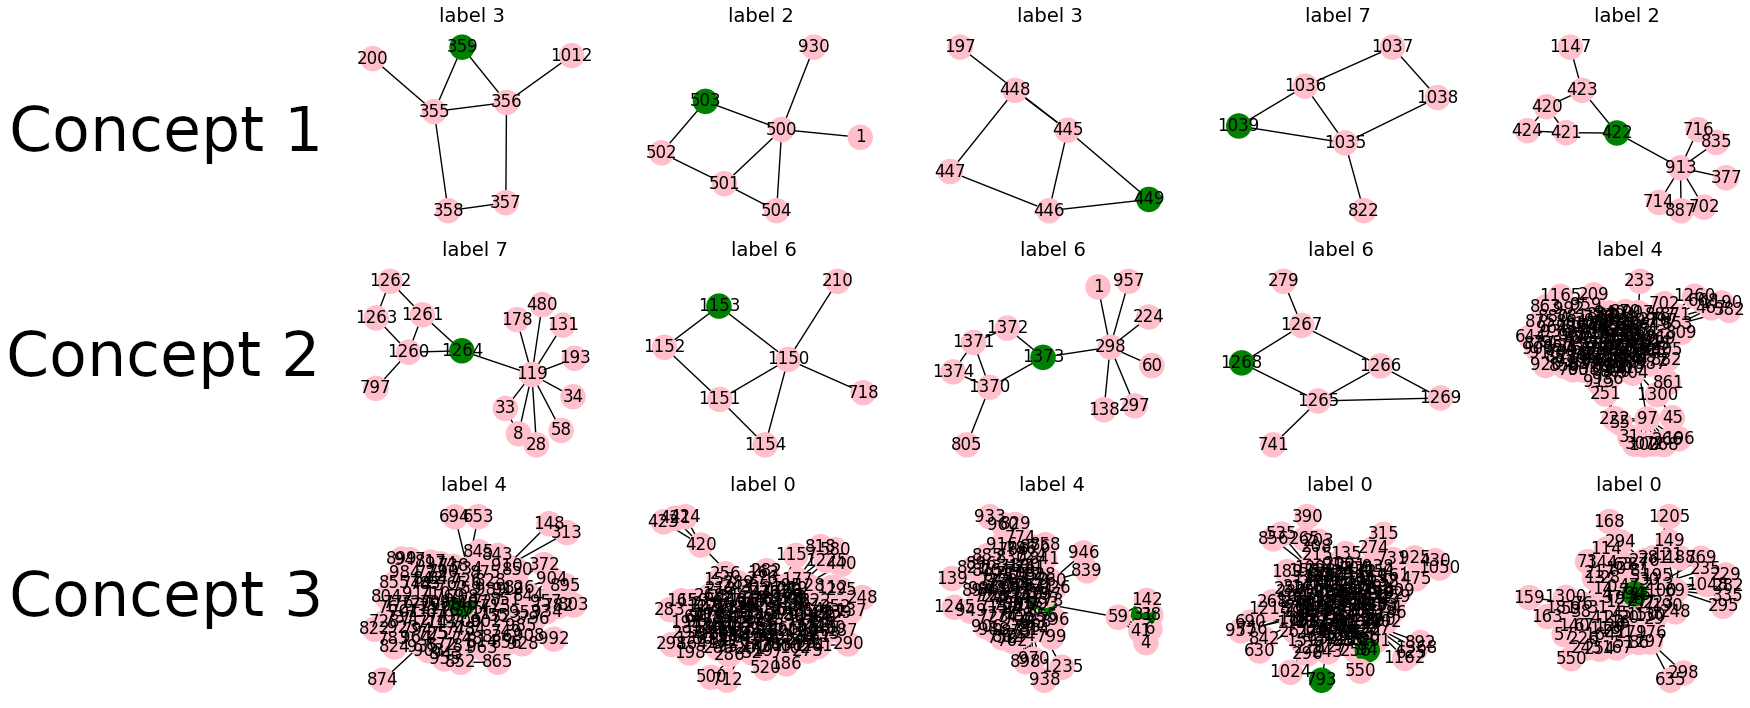
\includegraphics[width=0.75\textwidth]{figures/SGC-BA-Community}
    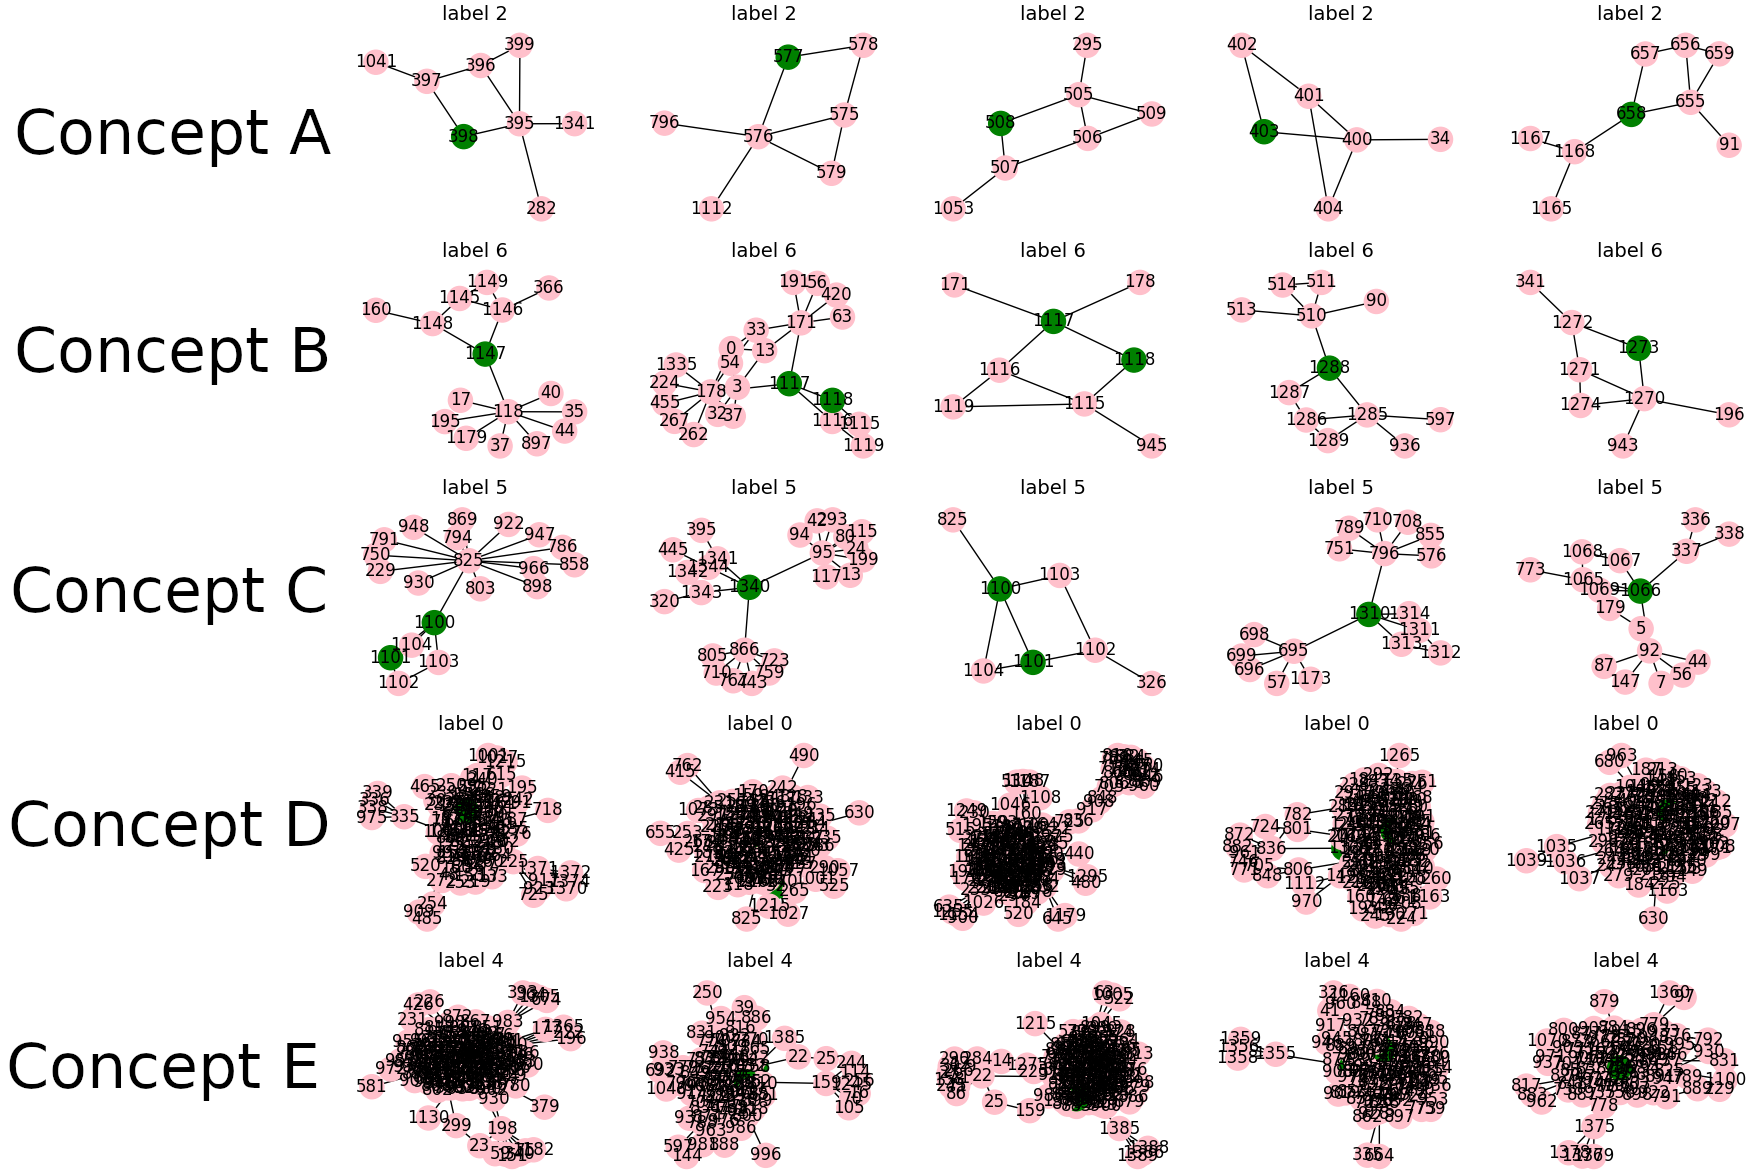
\includegraphics[width=0.75\textwidth]{figures/GCN-BA-Community}
    \caption{Comparison of SGC and GCN concepts for BA Community demonstrating the poor graph structural inference of SGC. The numbered concepts are a subset of SGC concepts and the lettered concepts are GCN concepts. The colour scheme is the same as fig. \ref{fig:GCN-BA-Shapes}.}
    \label{fig:BA-Community}
\end{figure}

Figure \ref{fig:BA-Community} highlights the inability of SGC to accurately discern graph structure where GCN demonstrate accurate graph structure discernment.
Concepts 1, 2 and 3 demonstrate the purer concepts for SGC trained on BA Community and Concepts A to E represent the equivalent concepts for GCN on BA Community.

As discussed SGC may be able to identify graph structure, as shown in concepts 1 and 2, however concept 1 highlights the fact that SGC cannot determine which part of the graph structure a node is.
Comparatively concepts A, B and C show a similar situation except consistent labels across the concept.

Furthermore, concept 2 includes a Barabasi-Albert subgraph, this is likely due to the similarity in node features for the second community\footnote{labels 4, 5, 6 and 7.} resulting in SGC treating them as the same.
In comparison GCN can distinguish between different communities as shown by concepts A and B which represent the same node in the house motif but different communities.
And GCN is able to discern between members in the same community demonstrated by concepts B and C.

This erroneous behaviour is not standard as concept 3 highlights how the Barabasi-Albert subgraphs from separate communities are grouped together.
GCN does treat the two communities different regardless of structural similarity which is clear in concepts D and E.

Overall SGC is able to infer basic graph structure or group nodes into communities but is unable to achieve fine-grained inference.
Though particularly apparent in BA Community these behaviours of SGC are likely to effect the performance on other datasets.

\subsection{Summary}
The low accuracy of SGC means that the data present in tables \ref{tab:SGC-completeness} and \ref{tab:SGC-purity} does not carry much meaning.
However, table \ref{tab:SGC-completeness} does suggest that SGC does not produce useful concepts even though table \ref{tab:SGC-purity} suggests that these concepts are coherent.

When looking at the concepts produce it is clear that SGC is not a capable GNN for synthetic datasets.
Figures \ref{fig:SGC-BA-Shapes} and \ref{fig:BA-Community} highlight how the relatively good purity and completeness scores do not relate to useful concepts.
The linearisation of GCN clearly does not maintain the graph capabilities of GCN contrary to the results and claims of \textit{Wu et al.}.

Considering the large parameter disparity and adjusting SGC to compensate does not improve the performance.
This suggests that non-linearity and trainable parameters are important at specific points during inference not on their own.

\section{Extensions}

\subsection{Evaluation}
All the extensions I explored focused on improving the ability of SGC or expanding the functionality of the model.
Therefore to evaluate the success of these attempts the models evaluated using the same techniques used in \ref{sec:evaluation}.
As these are extensions a smaller subset of the graph datasets are considered looking only at BA Shapes, as the best performing dataset, and BA Community, as the worst.

\subsection{SGC Graph Classification}
\paragraph{Motivation}
The datasets present in \textit{Magister et al.}\cite{magister2021gcexplainer} include 2 real world datasets that focus on graph classification.
As discussed in \Sref{sec:datasets} these graph classification datasets are also inductive rather than transductive which provides another test of the capabilities of SGC.
Furthermore, though \Sref{sec:comp-acc} suggests SGC performs poorly, this could be because of the synthetic nature of the datasets.

\paragraph{Prior work and implementation}
\textit{Wu et al.}\cite{wu2019simplifying} discuss graph classification for SGC suggesting that it can substitute GCN in a deep graph convolutional neural network as proposed by \note{name needed}\note{citation needed}.
However, \textit{Magister et al.} utilise pooling on the graph node representations after GCN to classify graphs. As this latter method is easier to implement and allows for a fairer comparison between SGC and GCN this approach is chosen.
The resulting model is identical to the standard SGC model with addition of a pooling layer before the classifier.

The only problem posed is to concept extraction as this is done on a node level as suggested by \textit{Magister et al.}.
This is overcome by broadcasting the graph label to each of the nodes.
This allows the graphs to be combined into a disconnected forest of graphs and clustering can be carried out on this forest.
Calculation of concept scores and the visualisation of concept therefore remains the same.

\paragraph{Results}
\fig{SGC-Mutagenicity}{Concepts from SGC and GCN for Mutagenicity comparing the complexity of the inferred graph structure. The numbered concepts are a subset of SGC concepts and the lettered concepts are a subset of GCN. The colour scheme matches standard chemical colours\note{citation needed}.}

Tables \ref{tab:SGC-acc}, \ref{tab:SGC-completeness} and \ref{tab:SGC-purity} already include the results achieved by SGC.
The same quantitative analysis presented in \Sref{sec:quant} can be applied to the results achieved by SGC.
This unfortunately suggests that the source of the graph data is not the issue, even though SGC performed well on Planetoid\cite{Fey/Lenssen/2019}.
As discussed in \Sref{comp-acc} the cause for the discrepancy is due to Planetoid\cite{Fey/Lenssen/2019} being focused on node representation.
Comparatively, Mutagenicity is both node representation and graph structure focused due to the nature of molecules.

Figure \ref{fig:SGC-Mutagenicity} further shows why SGC does not match the accuracy achieved by GCN.
Concepts 1, 2 and 3 focus on the inclusion of a single atom or small molecule structure wheres A, B and C demonstrate complex multi-atom structures.
Concepts 1 and 2 suggest some form of structure being identified however this is not consistent in comparison to A and B.
Concept 3 highlights the focus on grouping by atom as the major common component is the inclusion of the chlorine atom.
In comparison, concept C highlights how GCN is able to identify very large structures, here two cyclic rings are consistently identified.

\subsection{SGC and GCN Mixed Model}

\error{Need to implement mutual information to properly analyse compatibility.}

\paragraph{Motivation}
SGC is directly derived from GCN, the derivation provided in \Sref{sec:SGC}, using the same graph filter.
The benefit of SGC is to reduce the complexity of GCN and the cost of training by pre-computing the graph operation.
Though for the presented datasets in \Sref{sec:datasets} the improvement on cost and reduction in parameters is not significant larger datasets may create a larger benefit.
However, due to the low accuracy of SGC some aspects of GCN must required for high accuracy, therefore a mixture of both should yield a high accuracy model with pre-computation.

\paragraph{Implementation}

\paragraph{Results}

\subsection{JumpKnowledge style SGC}
\label{sec:Jump-SGC}

\paragraph{Motivation}
As discussed in \Sref{sec:concept-analysis} SGC does not have influence on the node representations during message passing.
SGC, of degree $k$, therefore has to infer graph structure from the aggregated node representations of all neighbouring nodes within $k$ hops.
Therefore the reason for the low accuracy and poor graph structure awareness may not be due to the linearity.
GCN is able to manipulate node representations between graph convolutions and can therefore further distinguish graph structure by potentially amplifying or damping differences between nodes.

For these reasons I propose \emph{jump-SGC}(JSGC) which provides the classifier with node representations from each degree of the pre-computation.
A fully-connected layer is added before the classifier to reduce the concatenated node representations into a single node representation.
This allows for JSGC to effectively manipulate the node representations though these manipulations do not have an impact on the application of the graph filter.
This idea mimics the \emph{jumping knowledge networks} (JCNs) proposed by \textit{Xu et al.}\cite{xu2018representation} hence the name ``jump''.

\paragraph{Prior work and Implementation}
\textit{Xu et al.}\cite{xu2018representation} identify the drawbacks of node aggregation in accurately representing a nodes neighbourhood.
It specifically identifies the effect on graph structure awareness this has making the method ideal for SGC.
The motivation for JCNs is the node aggregation methods used resulted in neighbourhood influence similar to a random walk rather than a uniform influence.
As a solution they propose aggregating the the node representations after successive neighbourhood aggregation layers together.
Three main methods of aggregation are proposed but given the small size of the datasets the proposed concatenation method is best suited.

By concatenating successive neighbourhood aggregations and then reducing the dimensionality to a single node representation uniform influence can be achieved.
This is because detail present in the closer neighbourhoods can be combined with the wider awareness of the more receptive neighbourhoods.
Rather than missing larger structure awareness or missing detail JCNs allow for an analysis of both.

For JSGC this leads to two changes to the model and pre-computation.
During pre-computation successive applications of the normalised filter are concatenated together.
A fully-connected layer is then added to the standard SGC to reduce this concatenated representation space to the standard representation space.
During this stage JSGC is able to infer more complex graph structure than SGC.
To combine this with the classifier a single non-linear rectified linear unit layer is introduced.
This non-linearity remains constant regardless of how the model scales and therefore the added potential benefits of the single non-linear layer is deemed negligible.

\paragraph{Results}

\begin{table}
    \centering
    \begin{tabular}{c|c|cc}
        \textbf{Dataset} & \textbf{JSGC} & \textbf{SGC} & \textbf{GCN} \\
        \midrule
        BA Shapes       & 78.2\% $\pm$ 3.2 & 61.4\% $\pm$ 3.3 & 98.0\% $\pm$ 2.2 \\
        BA Community    & $\pm$ & 20.6\% $\pm$ 1.5 & 86.3\% $\pm$ 3.3 \\
    \end{tabular}
    \caption{Test accuracy in \% of JSGC on a subset of synthetic datasets using the hyperparameters in table \note{reference when complete}. Each experiment is run until convergence. Results from SGC and GCN are provided as a comparison.}
    \label{tab:SJGC-acc}
\end{table}


\begin{table}[h]
    \centering
    \captionsetup{width=.9\textwidth}
    \begin{tabular}{c|c|cc}
        \textbf{Dataset} &
        \textbf{JSGC} &
        \textbf{SGC} &
        \textbf{GCN} \\
        \midrule
        BA Shapes       & 0.943 & 0.882 & 0.964 \\
        BA Community    & \textbf{0.704} & 0.264 & 0.678 \\
    \end{tabular}
    \caption{Concept completeness scores of JSGC on a subset of the synthetic datasets using the hyperparameters in table \ref{tab:JSGC-params} compared to the completeness scores of the equivalent SGC and GCN models. Each model is run until convergence and the best performing model selected for concept extraction.}
    \label{tab:JSGC-completeness}
\end{table}


\begin{table}[h]
    \centering
    \captionsetup{width=.9\textwidth}
    \begin{tabular}{c|ccc|cc}
        \multirow{2}{*}{\textbf{Dataset}} &
        \multicolumn{3}{c|}{\textbf{JSGC}} & \\
        & \textbf{Max.} & \textbf{Min.} & \textbf{Mean} & 
        \multirow{-2}{*}{\textbf{SGC}} &
        \multirow{-2}{*}{\textbf{GCN}}\\
        \midrule
        BA Shapes       & 0.0 & 0.0 & 0.0 (2) & 0.8 (5) & 0.000 (4) \\
        BA Community    & 4.0 & 16.0 & 9.4 (7) & 4.0 (4) & 5.600 (3) \\
    \end{tabular}
    \caption{Concept purity of JSGC on a subset of the synthetic datasets using the hyperparameters in table \ref{tab:JSGC-params} compared to the average purity achieved by the equivalent SGC and GCN model. The brackets represent the number of concepts considered for purity, as per \Sref{sec:evaluation} these are graphs with less than 13.}
    \label{tab:JSGC-purity}
\end{table}



Tables \ref{tab:JSGC-acc}, \ref{tab:JSGC-completeness} and \ref{tab:JSGC-purity} show the results achieved by JSGC on the datasets analysed in \Sref{sec:comp-concept}.
Overall these demonstrate that JSGC does outperform SGC significantly and is more comparable to GCN.
The accuracy achieved by JSGC is still lower than the the 95\% suggested by \textit{Ying et al.}\cite{ying2019gnnexplainer} but significantly better.
This improvement is seen in table \ref{tab:JSGC-completeness} as the completeness scores are closer to 1 with BA Community producing better performing concepts than GCN.\footnote{This is partially a result of the concept parameters used. The high score signifies that good concepts are being utilised by the model but in this case the model still does not appear to be quite capable enough.}
The purity presented in table \ref{tab:JSGC-purity} is higher though more concepts were considered and BA Community is a very complex graph.

\fig{JSGC-BA-Community}{A subset of concepts from JSGC for BA Community demonstrating the improved graph structure awareness. The concepts are chosen to represent the GCN concepts presented in \ref{fig:BA-Community}. The colour scheme is the same as fig \ref{fig:GCN-BA-Shapes}.}

Figure \ref{fig:JSGC-BA-Community} highlights the improvements that JSGC has made compared to SGC.
Comparing these concepts to those achieved by GCN presented in figure \ref{fig:BA-Community} shows a clear improvement.
Concepts 1 to 5 in fig. \ref{fig:JSGC-BA-Community} can be directly mapped to A to E in fig. \ref{fig:JSGC-BA-Community}.\footnote{A similar direct mapping was also achieved for BA Shapes.}
JSGC is now able to distinguish between the two communities highlighted by concepts 1 \& 2 and 3 \& 4.
Furthermore, within a community JSGC correctly distinguishes between the different nodes as concept 2, 3 and 4 show.
Most importantly all concepts, except for concept 1, show consistent labelling throughout, particularly in concept 3 where all nodes are ``outside''\footnote{See \Sref{sec:concept-analysis}.} nodes.

Clearly JSGC has comparable graph structure awareness as GCN and does not require the non-linearity of GCN to achieve this.
The lower accuracy of JSGC still suggests that there are elements of GCN that are important to its success and generally GRL.
However, further studies into the importance of non-linearity in GRL is required.

